\documentclass[12pt, a4paper, oneside, openany]{report}

% --- Packages ---
\usepackage[a4paper, margin=0.8in]{geometry}
\usepackage{fontspec}
\usepackage{xcolor}
\usepackage{tikz}
\usetikzlibrary{shapes.geometric, arrows.meta, positioning, calc}
\usepackage{longtable}
\usepackage{array}
\usepackage{titlesec}
\usepackage{tocloft}
\usepackage{caption}
\usepackage{graphicx}
\usepackage{microtype}
\usepackage{fancyhdr}
\usepackage[most]{tcolorbox}
\usepackage{listings}
\usepackage[colorlinks=true, linkcolor=black, citecolor=black, urlcolor=black, filecolor=black]{hyperref}

% --- Font Customization (TeX Gyre Pagella Font Family) ---
\setmainfont{TeX Gyre Pagella}

% --- Footer Page Numbering Setup (Centered Footer Only, No Header Rules) ---
\pagestyle{fancy}
\fancyhf{}
\cfoot{\thepage}
\renewcommand{\headrulewidth}{0pt}
\renewcommand{\footrulewidth}{0pt}

% Ensure plain style (used on Chapter first pages) also uses centered footer page numbering
\fancypagestyle{plain}{
  \fancyhf{}
  \cfoot{\thepage}
  \renewcommand{\headrulewidth}{0pt}
  \renewcommand{\footrulewidth}{0pt}
}

% --- Line Spacing & Hyphenation Rules ---
\linespread{1.3}

% --- Code Snippet Styling (Eye-Friendly Grey TColorBox + GitHub Green Comments) ---
\definecolor{codebg}{RGB}{246,248,250}
\definecolor{codeborder}{RGB}{210,215,220}
\definecolor{commentgreen}{RGB}{46,125,50}   % GitHub green for comments
\definecolor{keywordblue}{RGB}{5,80,174}    % GitHub blue for keywords
\definecolor{stringred}{RGB}{163,21,21}     % GitHub red for strings

\tcbuselibrary{listings, skins}

\newtcblisting{codeblock}[1][]{
  enhanced,
  colback=codebg,
  colframe=codeborder,
  arc=5pt,
  boxrule=0.8pt,
  left=10pt, right=10pt, top=8pt, bottom=8pt,
  listing only,
  listing options={
    basicstyle=\ttfamily\scriptsize\color{black},
    keywordstyle=\color{keywordblue}\bfseries,
    commentstyle=\color{commentgreen}\itshape,
    stringstyle=\color{stringred},
    breaklines=true,
    breakatwhitespace=false,
    columns=fullflexible,
    keepspaces=true,
    showstringspaces=false
  },
  #1
}

% --- Inline Code Specification (Soft Eye-Friendly Slate Grey + Slate Navy Text + Auto Next-Line Wrap) ---
\definecolor{inlinebg}{RGB}{241,243,245}
\definecolor{inlinetext}{RGB}{24,43,73}

\newcommand{\code}[1]{%
  \leavevmode\penalty0%
  \begingroup
  \setlength{\fboxsep}{2pt}%
  \ttfamily\small\color{inlinetext}%
  \colorbox{inlinebg}{\vphantom{Ag}\detokenize{#1}}%
  \endgroup
}
\pdfstringdefDisableCommands{\def\code#1{#1}}

% --- Chapter & Section Formatting Rules ---
% Chapters: Centered, Bold, 18pt, ALL CAPS (starts immediately on next page, no blank gaps)
\titleformat{\chapter}[block]
  {\centering\normalfont\fontsize{18pt}{22pt}\bfseries}
  {\thechapter. }
  {0pt}
  {}
\titlespacing*{\chapter}{0pt}{0pt}{20pt}

% Sections (Subheadings): Bold, 14pt
\titleformat{\section}[block]
  {\normalfont\fontsize{14pt}{18pt}\bfseries}
  {\thesection\quad}
  {0pt}
  {}
\titlespacing*{\section}{0pt}{14pt}{8pt}

% Subsections: Bold, 12.5pt
\titleformat{\subsection}[block]
  {\normalfont\fontsize{12.5pt}{16pt}\bfseries}
  {\thesubsection\quad}
  {0pt}
  {}
\titlespacing*{\subsection}{0pt}{10pt}{4pt}

% --- Table Spacing & Column Alignments ---
\renewcommand{\arraystretch}{1.4}
\setlength{\tabcolsep}{5pt}

% Column Types with RaggedRight to prevent awkward justification in cells
\newcolumntype{L}[1]{>{\raggedright\arraybackslash}p{#1}}
\newcolumntype{C}[1]{>{\centering\arraybackslash}p{#1}}

% --- TOC Formatting ---
\renewcommand{\cftchapfont}{\bfseries}
\renewcommand{\cftchappagefont}{\bfseries}

\begin{document}

% ==========================================================
% FRONT PAGE (DYNAMIC BORDER WITH ROUNDED CORNERS)
% ==========================================================
\begin{titlepage}
\begin{tikz}[remember picture, overlay]
  \draw[line width=1.5pt, black, rounded corners=8pt] 
    ($(current page.north west) + (0.5in, -0.5in)$) 
    rectangle 
    ($(current page.south east) + (-0.5in, 0.5in)$);
\end{tikz}

\vspace*{0.8in}
\begin{center}
  {\fontsize{26pt}{32pt}\bfseries TV-NEWSHUB}\\[0.2in]
  {\fontsize{14pt}{18pt}\bfseries COMPREHENSIVE ENGINEERING ARCHITECTURE, LOW-LEVEL DESIGN (LLD) \& INTERVIEW GUIDE}\\[0.4in]
  
  \vspace{0.3in}
  
\includegraphics[width=2.2in]{../../public/logo.png}\\[0.4in]
  
  \vspace{0.2in}
  {\fontsize{12pt}{15pt}\bfseries TECHNICAL DEEP-DIVE \& SYSTEMS DESIGN DOCUMENTATION}\\[0.1in]
  {\fontsize{11pt}{14pt}Target Platforms: Android TV | Google TV | Fire TV OS}\\[0.05in]
  {\fontsize{11pt}{14pt}Framework: React Native TVOS v0.83}\\[0.05in]
  {\fontsize{11pt}{14pt}Current Release: Version v0.0.5}\\[0.6in]

  \vfill

  \begin{tabular}{|L{2.2in}|L{3.8in}|}
    \hline
    \textbf{Document Type} & Comprehensive Interview-Ready Engineering Wiki \\ \hline
    \textbf{Maintainer} & Biraj2004 (TV-NewsHub Repository Lead) \\ \hline
    \textbf{License} & Apache License 2.0 \\ \hline
    \textbf{Target Resolution} & 1080p Full HD / 4K UHD Hardware Decoded Streams \\ \hline
  \end{tabular}

  \vspace{0.5in}
\end{center}
\end{titlepage}

% ==========================================================
% TABLE OF CONTENTS
% ==========================================================
\tableofcontents
\newpage

% ==========================================================
% CHAPTER 1: EXECUTIVE SUMMARY & ARCHITECTURAL VISION
% ==========================================================
\chapter{EXECUTIVE SUMMARY \& ARCHITECTURAL VISION}

\section{Problem Statement \& OTT Challenge}
Linear news broadcasting on Smart TV platforms faces significant technical challenges:
\begin{enumerate}
  \item \textbf{Endpoint Fragility}: Direct HLS feeds (\code{.m3u8}) hosted on Akamai or CloudFront CDNs frequently rotate security tokens or expire.
  \item \textbf{CORS \& Embed Trapping}: Broadcaster web widgets (e.g., Zee News, ABP Live) rely on cross-origin iframe security or complex DOM script rendering, failing inside traditional native video wrappers like \code{ExoPlayer}.
  \item \textbf{YouTube Live Stream ID Shifts}: News networks regularly cycle YouTube Live stream IDs when switching live broadcast segments or breaking news programs.
  \item \textbf{Hardware Constraints}: Smart TV microprocessors operate on low-power ARM v7/v8 or x86 chipsets with strict memory limits (1GB–2GB RAM) and limited software video decoding threads.
\end{enumerate}

\section{System Solution: TV-NewsHub}
\code{TV-NewsHub} solves these challenges through a \textbf{3-tier dynamic resolution waterfall}, an \textbf{in-memory 5-minute TTL caching layer}, a \textbf{smart TV D-Pad remote focus engine}, and \textbf{automated Layer-2 DOM consent handling}.

\section{Key Metric \& Reliability Targets}

\begin{longtable}{|L{1.5in}|L{1.5in}|L{3.1in}|}
  \hline
  \textbf{Engineering Metric} & \textbf{Target Goal} & \textbf{Production Mechanism} \\ \hline
  \endhead
  \hline
  \endfoot
  Stream Uptime & 100\% Availability & 3-Tier Dynamic Waterfall (HLS $\rightarrow$ Embed $\rightarrow$ YouTube) \\ \hline
  Video Quality & 1080p Full HD (3.9 Mbps) & \code{capLevelToPlayerSize: false} + \code{hls.currentLevel = max} \\ \hline
  Remote Input Latency & $< 16$ms (60 FPS) & Native Android \code{View} focus nodes + \code{FocusGrabber} overlay \\ \hline
  Network Memory Leaks & 0 Leaked Connections & 10-Second \code{AbortController} timeouts on all fetch calls \\ \hline
  Consent Interruption & 0 User Clicks Needed & Layer-1 cookie sandboxing + Layer-2 DOM MutationObserver \\ \hline
\end{longtable}

% ==========================================================
% CHAPTER 2: TECHNOLOGY STACK & TRADE-OFF ANALYSIS
% ==========================================================
\chapter{TECHNOLOGY STACK \& TRADE-OFF ANALYSIS}

\section{Core Stack Component Matrix}

\begin{longtable}{|L{1.4in}|L{2.2in}|L{2.5in}|}
  \hline
  \textbf{Subsystem} & \textbf{Selected Technology} & \textbf{Engineering Trade-Off Rationale} \\ \hline
  \endhead
  \hline
  \endfoot
  Runtime & React Native TVOS \code{v0.83.0} & Native Android TV remote focus nodes without Java boilerplate. \\ \hline
  UI Framework & React Native \code{v19.2.0} & Declarative component state with high-performance 60 FPS flex layout. \\ \hline
  WebView Engine & \code{react-native-webview} & System Chromium engine executing JavaScript DOM auto-clickers. \\ \hline
  HLS Engine & \code{Hls.js v1.5.0} & Allows JavaScript override of manifest bitrate selection. \\ \hline
  YouTube Resolver & \code{react-native-}\allowbreak\code{youtube-iframe} & Embeds YouTube iframe with custom forwardRef imperative handles. \\ \hline
  Cookie Engine & \code{@react-native-}\allowbreak\code{cookies/cookies} & Direct native C++ cookie injection for domain sandboxing. \\ \hline
  Storage & \code{@react-native-}\allowbreak\code{async-storage} & Persistent key-value storage for last-watched channel memory. \\ \hline
\end{longtable}

\section{Detailed Framework Evaluation Matrix}

\begin{longtable}{|L{1.3in}|L{1.6in}|L{1.6in}|L{1.4in}|}
  \hline
  \textbf{Evaluation Criteria} & \textbf{React Native TVOS} & \textbf{Native Kotlin (Leanback)} & \textbf{Flutter for TV} \\ \hline
  \endhead
  \hline
  \endfoot
  Web Share Widget Support & \textbf{Excellent} (Native WebView) & Poor (WebView lifecycle lag) & Poor (Compositing drops) \\ \hline
  D-Pad Remote Handling & \textbf{Excellent} (Native focus) & Excellent (Leanback SDK) & Fair (Focus tree bugs) \\ \hline
  Bitrate Forcing Control & \textbf{Excellent} (Hls.js API) & Requires C++ ExoPlayer mod & Difficult \\ \hline
  Build \& Release Speed & \textbf{Fast} (Universal JS bundle) & Slow (Java compilation) & Medium \\ \hline
\end{longtable}

% ==========================================================
% CHAPTER 3: STREAM PROVIDER ARCHITECTURE & DYNAMIC FALLBACK
% ==========================================================
\chapter{STREAM PROVIDER ARCHITECTURE \& DYNAMIC FALLBACK}

\section{3-Tier Stream Waterfall Architecture}

\begin{center}
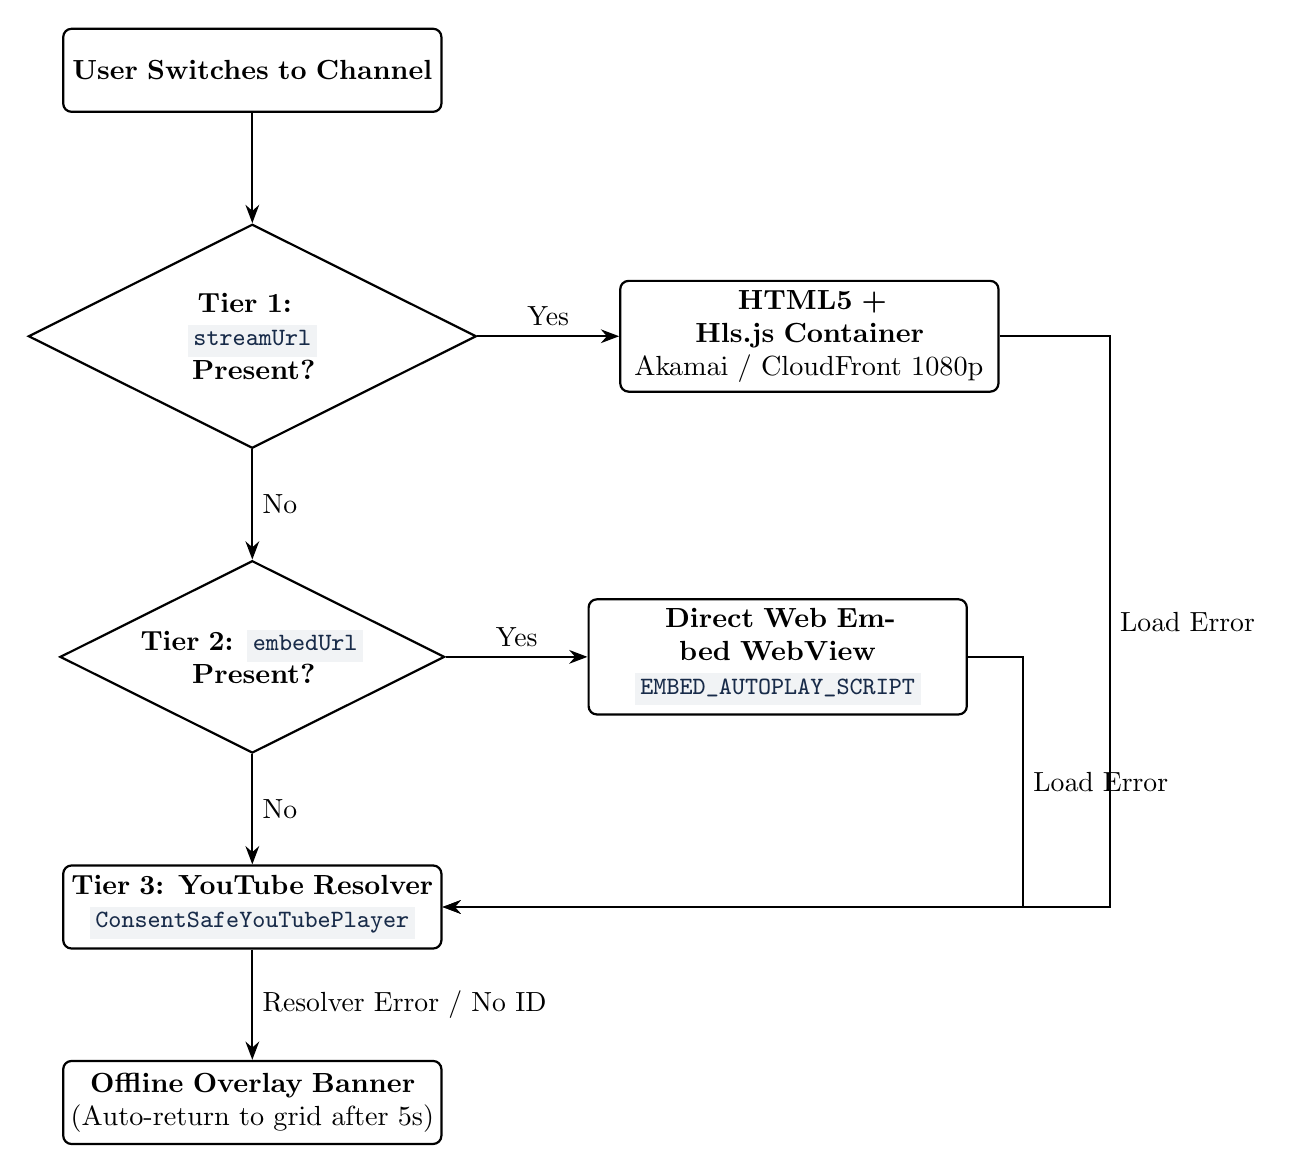
\begin{tikzpicture}[node distance=1.4cm and 1.8cm, auto, >=Stealth]
  \tikzstyle{block} = [rectangle, draw=black, thick, text width=13em, align=center, rounded corners=3pt, minimum height=3em, fill=white]
  \tikzstyle{decision} = [diamond, draw=black, thick, text width=8em, align=center, aspect=2, fill=white]

  \node [block] (start) {\textbf{User Switches to Channel}};
  \node [decision, below=of start] (tier1) {\textbf{Tier 1: \code{streamUrl} Present?}};
  \node [block, right=of tier1] (hls) {\textbf{HTML5 + Hls.js Container}\\Akamai / CloudFront 1080p};
  \node [decision, below=of tier1] (tier2) {\textbf{Tier 2: \code{embedUrl} Present?}};
  \node [block, right=of tier2] (embed) {\textbf{Direct Web Embed WebView}\\\code{EMBED_AUTOPLAY_SCRIPT}};
  \node [block, below=of tier2] (tier3) {\textbf{Tier 3: YouTube Resolver}\\\code{ConsentSafeYouTubePlayer}};
  \node [block, below=of tier3] (offline) {\textbf{Offline Overlay Banner}\\(Auto-return to grid after 5s)};

  \draw [->, thick] (start) -- (tier1);
  \draw [->, thick] (tier1) -- node[above] {Yes} (hls);
  \draw [->, thick] (tier1) -- node[right] {No} (tier2);
  \draw [->, thick] (hls.east) -- ++(1.4cm,0) |- node[near start, right] {Load Error} (tier3.east);
  \draw [->, thick] (tier2) -- node[above] {Yes} (embed);
  \draw [->, thick] (tier2) -- node[right] {No} (tier3);
  \draw [->, thick] (embed.east) -- ++(0.7cm,0) |- node[near start, right] {Load Error} (tier3.east);
  \draw [->, thick] (tier3) -- node[right] {Resolver Error / No ID} (offline);
\end{tikzpicture}
\end{center}

\section{Dynamic Fallback Implementation (\code{useYoutubeFallback})}
When \code{PlayerScreen.tsx} encounters a loading failure on Tier 1 (HLS) or Tier 2 (Embed), instead of presenting an offline error dialog immediately, it executes the \code{handlePrimaryStreamError()} callback:

\begin{codeblock}
// Primary Stream Failure Handler in PlayerScreen.tsx
const handlePrimaryStreamError = useCallback((errorMessage: string) => {
  if (currentChannel.youtubeChannelId && !useYoutubeFallback) {
    console.log('[PlayerScreen] Primary stream failed. Fallback to YouTube...');
    setUseYoutubeFallback(true);
  } else {
    setPlaybackError(errorMessage);
  }
}, [currentChannel, useYoutubeFallback]);
\end{codeblock}

If \code{youtubeChannelId} exists, \code{useYoutubeFallback} transitions to \code{true}, dynamically unmounting the broken WebView and mounting \code{ConsentSafeYouTubePlayer} seamlessly!

% ==========================================================
% CHAPTER 4: NETWORK MANAGEMENT & EDGE CASE HANDLING
% ==========================================================
\chapter{NETWORK MANAGEMENT \& EDGE CASE HANDLING}

\section{Network Request Lifecycle \& Safety Mechanisms}

\begin{longtable}{|L{1.5in}|L{2.3in}|L{0.8in}|L{1.5in}|}
  \hline
  \textbf{Network Operation} & \textbf{Endpoint / Target} & \textbf{Timeout} & \textbf{Caching Strategy} \\ \hline
  \endhead
  \hline
  \endfoot
  YouTube Live HTML Scan & \code{https://www.youtube.com/channel/<ID>/live} & 10,000ms & 5-Min Memory Map (\code{CACHE_TTL_MS}) \\ \hline
  YouTube RSS Feed Fallback & \code{https://www.youtube.com/feeds/videos.xml} & 10,000ms & 5-Min Memory Map (\code{CACHE_TTL_MS}) \\ \hline
  Google Connectivity Probe & \code{https://clients3.google.com/generate_204} & 3,000ms & Event-based (NetInfo trigger) \\ \hline
  GitHub Release Updater & \code{https://api.github.com/repos/.../releases} & 4,000ms & Single execution on app mount \\ \hline
\end{longtable}

\section{Subsystem Failure Modes \& Edge Case Matrix (FMEA)}

\begin{longtable}{|L{1.4in}|L{1.8in}|L{2.9in}|}
  \hline
  \textbf{Subsystem Component} & \textbf{Potential Edge Case / Failure} & \textbf{Automated Handling Strategy} \\ \hline
  \endhead
  \hline
  \endfoot
  Tier 1 HLS Stream & CDN Token Expiry / HTTP 403 / Manifest Error & Triggers \code{handlePrimaryStreamError()} $\rightarrow$ Falls back to YouTube. \\ \hline
  Tier 2 Embed Player & CORS Iframe Blocking / Cross-Domain Policy & Loaded directly via WebView \code{source=\{\{ uri \}\}} with page JS injection. \\ \hline
  Tier 3 YouTube Resolver & YouTube Changes Live URL Structure & Strategy A (HTML regex) fails over to Strategy B (UULV RSS XML parsing). \\ \hline
  YouTube Cookie Dialog & GDPR Popup Blocks Video Playback & Layer 1 \code{CONSENT=YES+} cookie set + Layer 2 DOM MutationObserver click. \\ \hline
  D-Pad Remote Focus & WebView swallows D-Pad key events & Invisible \code{FocusGrabber} Pressable overlay (\code{zIndex: 1}) retains focus. \\ \hline
  Network Disconnection & Wi-Fi drops during video playback & \code{useNetworkStatus} triggers \code{NoInternetScreen} full overlay. \\ \hline
  App Update Check & GitHub API Rate Limit / Network Error & Silent exception catch (\code{__DEV__} log only); application launches normally. \\ \hline
\end{longtable}

% ==========================================================
% CHAPTER 5: BRANDING, LOGO ASSETS & UI SYSTEM
% ==========================================================
\chapter{BRANDING, LOGO ASSETS \& UI SYSTEM}

\section{Static Logo Asset Bundling Strategy}
Smart TV environments cannot rely on asynchronous web images for channel logos due to latency and missing image placeholders. \code{TV-NewsHub} bundles high-resolution \code{.webp} logos directly inside the application package (\code{public/channel-logos/}).

To avoid dynamic \code{require()} calls (which break in React Native's Metro bundler), \code{src/utils/logoHelper.ts} provides a pre-compiled lookup table:

\begin{codeblock}
// Pre-compiled Channel Logo Image Require Lookup Map
const LOGO_MAP: Record<string, any> = {
  'republic-bangla': require('../../public/channel-logos/India/Bengali/republic_bangla.webp'),
  'abp-ananda': require('../../public/channel-logos/India/Bengali/abp_ananda.webp'),
  'tv9-bangla': require('../../public/channel-logos/India/Bengali/tv9_bangla.webp'),
  'news18-bangla': require('../../public/channel-logos/India/Bengali/news18_bangla.webp'),
  'calcutta-news': require('../../public/channel-logos/India/Bengali/calcutta_news.webp'),
  'zee-24-ghanta': require('../../public/channel-logos/India/Bengali/zee_24_ghanta.webp'),
};
\end{codeblock}

\section{Smart TV Focus Zoom \& Spatial Visual Engine}
When a user navigates between channel tiles on the home screen:
\begin{enumerate}
  \item Focused channel tile scales up smoothly by \textbf{\code{1.05x}} via React Native \code{Animated} or scale transform props.
  \item Displays a high-contrast \textbf{\code{#ffffff} 3px border} with a 12px border radius.
  \item Non-focused channel tiles remain at \code{opacity: 0.8} to emphasize spatial visual hierarchy across the 10-foot viewing distance.
\end{enumerate}

% ==========================================================
% CHAPTER 6: IN-APP OTA UPDATER ARCHITECTURE
% ==========================================================
\chapter{IN-APP OTA UPDATER ARCHITECTURE}

\section{GitHub Release Check Lifecycle}
In \code{src/utils/updateChecker.ts}, the application silently checks for new production releases on startup without blocking the user:

\begin{center}
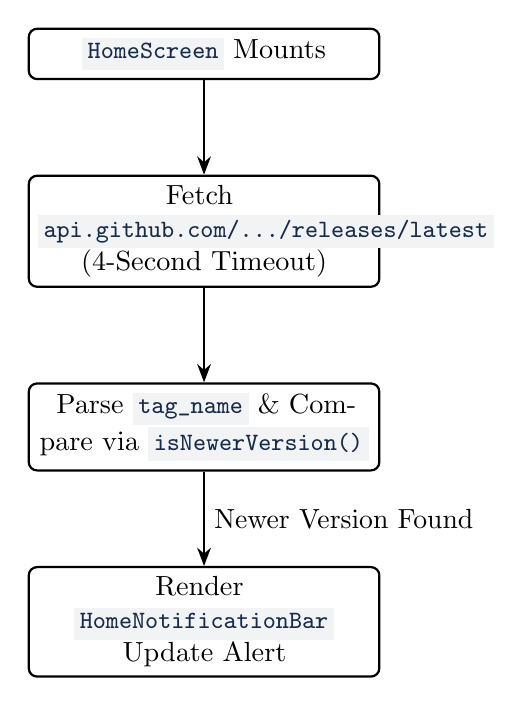
\begin{tikzpicture}[node distance=1.2cm and 1.5cm, auto, >=Stealth]
  \tikzstyle{block} = [rectangle, draw=black, thick, text width=12em, align=center, rounded corners=3pt, fill=white]

  \node [block] (start) {\code{HomeScreen} Mounts};
  \node [block, below=of start] (fetch) {Fetch \code{api.github.com/.../releases/latest}\\(4-Second Timeout)};
  \node [block, below=of fetch] (parse) {Parse \code{tag_name} \& Compare via \code{isNewerVersion()}};
  \node [block, below=of parse] (banner) {Render \code{HomeNotificationBar} Update Alert};

  \draw [->, thick] (start) -- (fetch);
  \draw [->, thick] (fetch) -- (parse);
  \draw [->, thick] (parse) -- node[right] {Newer Version Found} (banner);
\end{tikzpicture}
\end{center}

\section{Version Comparison Logic (\code{isNewerVersion})}
The version comparator parses semantic version strings (e.g. \code{v0.0.5} vs \code{v0.0.3}) into numeric array components:

\begin{codeblock}
// Semantic Version Comparer Algorithm
function isNewerVersion(latest: string, current: string): boolean {
  if (!latest || !current) return false;
  const lParts = latest.split('.').map((p) => parseInt(p, 10) || 0);
  const cParts = current.split('.').map((p) => parseInt(p, 10) || 0);

  for (let i = 0; i < Math.max(lParts.length, cParts.length); i++) {
    const l = lParts[i] || 0;
    const c = cParts[i] || 0;
    if (l > c) return true;
    if (l < c) return false;
  }
  return false;
}
\endcodeblock

% ==========================================================
% CHAPTER 7: LOW-LEVEL DESIGN (LLD) & DESIGN PATTERNS
% ==========================================================
\chapter{LOW-LEVEL DESIGN (LLD) \& DESIGN PATTERNS}

\section{Software Design Pattern Map}

\begin{longtable}{|L{1.5in}|L{2.0in}|L{2.6in}|}
  \hline
  \textbf{Design Pattern} & \textbf{Implementation File} & \textbf{System Purpose} \\ \hline
  \endhead
  \hline
  \endfoot
  Strategy Pattern & \code{PlayerScreen.tsx} & Dynamically selects player renderer (HLS vs Embed vs YouTube). \\ \hline
  Proxy / Adapter Pattern & \code{ConsentSafeYouTubePlayer.tsx} & Wraps YouTube iframe with cookies \& \code{forcePlay()} handles. \\ \hline
  Observer Pattern & \code{useIdleTimer.ts} & Listens to D-Pad activity and auto-hides player controls after 4s. \\ \hline
  Flyweight / Lookup & \code{logoHelper.ts} & Pre-cached map of static WebP channel logo image requires. \\ \hline
\end{longtable}

\section{Complete Module Hierarchy Map}

\begin{codeblock}
src/
|-- components/
|   |-- ConsentSafeYouTubePlayer.tsx (Proxy player for YouTube embeds)
|   |-- ChannelTile.tsx             (Focused channel tile node)
|   |-- PlayerOverlay.tsx            (Translucent D-Pad UI overlay)
|   |-- HomeNotificationBar.tsx     (Breaking news / update status bar)
|   |-- CountryTabs.tsx             (Country filter chip row)
|   |-- LanguageTabs.tsx            (Language filter chip row)
|   +-- NoInternetScreen.tsx        (Full-screen network outage screen)
|-- data/
|   +-- countries/india.json         (Channel endpoint definitions)
|-- hooks/
|   |-- useLiveChannelResolver.ts   (YouTube live stream ID resolver)
|   |-- useIdleTimer.ts             (Overlay auto-hide timer hook)
|   +-- useNetworkStatus.ts         (NetInfo & Google 204 connectivity hook)
|-- screens/
|   |-- HomeScreen.tsx              (Grid channel catalog)
|   +-- PlayerScreen.tsx            (Full-screen video player & zapping)
+-- utils/
    |-- playerScripts.ts            (Extracted DOM autoplay & quality JS)
    |-- updateChecker.ts            (GitHub Releases OTA update checker)
    |-- sanitize.ts                 (XSS URL sanitizer)
    |-- storage.ts                  (AsyncStorage last-watched channel)
    +-- logoHelper.ts               (Local logo asset mapper)
\endcodeblock

% ==========================================================
% CHAPTER 8: PERFORMANCE OPTIMIZATION & BITRATE CONTROL
% ==========================================================
\chapter{PERFORMANCE OPTIMIZATION \& BITRATE CONTROL}

\section{Hls.js Buffer Depth \& Bitrate Forcing Configuration}
In \code{src/utils/playerScripts.ts}, \code{getHlsHtml()} overrides default Web Hls.js settings to prevent resolution drops on TV displays:

\begin{codeblock}
// Hls.js Buffer Memory Configuration & Bitrate Lock
var hls = new Hls({
  maxBufferLength: 60,            // 60-second video pre-buffer
  maxMaxBufferLength: 120,        // Max upper bound 2 minutes
  maxBufferSize: 60 * 1000 * 1000, // 60 MB buffer memory footprint
  maxBufferHole: 0.5,
  capLevelToPlayerSize: false,    // Ignore container DP size bounds
  startLevel: -1                  // Auto-detect then force max level
});
hls.on(Hls.Events.MANIFEST_PARSED, function() {
  if (hls.levels && hls.levels.length > 0) {
    hls.currentLevel = hls.levels.length - 1; // Lock to top 1080p bitrate
    hls.autoLevelCapping = -1;
  }
});
\endcodeblock

% ==========================================================
% CHAPTER 9: SECURITY ARCHITECTURE & PRIVACY ENGINEERING
% ==========================================================
\chapter{SECURITY ARCHITECTURE \& PRIVACY ENGINEERING}

\section{Security Controls Summary}
\begin{enumerate}
  \item \textbf{XSS Sanitization}: \code{sanitizeUrl()} strips characters (\code{[`'"\\<>]}) before template string insertion.
  \item \textbf{Cookie Domain Sandboxing}: \code{CookieManager.set()} scopes consent values exclusively to \code{.youtube.com} and \code{.google.com}.
  \item \textbf{Zero Secret Persistence}: No auth tokens or private credentials stored in \code{AsyncStorage}.
\end{enumerate}

% ==========================================================
% CHAPTER 10: BUILD PIPELINE & RELEASE EXPORT
% ==========================================================
\chapter{BUILD PIPELINE \& RELEASE EXPORT}

\section{ABI Architecture Splitting}

\begin{longtable}{|L{1.5in}|L{1.8in}|L{2.5in}|}
  \hline
  \textbf{Exported Release APK} & \textbf{Target CPU Architecture} & \textbf{Recommended Target Hardware} \\ \hline
  \endhead
  \hline
  \endfoot
  \code{TV-NewsHub-v0.0.5-universal.apk} & All Architectures (FAT APK) & Recommended for All Smart TVs \\ \hline
  \code{TV-NewsHub-v0.0.5-arm64-v8a.apk} & ARM 64-bit & Modern 4K Smart TVs \& Fire TV Stick 4K \\ \hline
  \code{TV-NewsHub-v0.0.5-armeabi-v7a.apk} & ARM 32-bit & Legacy HD Smart TVs \& Mi Box / Sticks \\ \hline
  \code{TV-NewsHub-v0.0.5-x86_64.apk} & Intel/AMD 64-bit & 64-bit Android Studio Emulators \\ \hline
  \code{TV-NewsHub-v0.0.5-x86.apk} & Intel/AMD 32-bit & 32-bit Android Studio Emulators \\ \hline
\end{longtable}

\section{Release Build Command}
\begin{codeblock}
# Android Release APK Compilation Command
cd android && gradlew.bat assembleRelease
\end{codeblock}

\end{document}
